% X. The classifier study (simulated). Three follow-up experiments, each
% pre-registered after E1-E6 were known (results/{classifier,hindsight,
% web_rankers}/PREREGISTERED.md): the classifier zoo and the real-trace
% router benchmark (track CLF), the hindsight-labelled router whose actions
% include read-ahead depth (HSR), and the web ranker alternatives (WRK); the
% MSRC light sample (E7) is in the appendix. Every verdict is a \dec macro
% computed by paper/decisions.py; synthetic accuracies are labelled
% synthetic; every disk hit ratio is paired with device work.
% Generated: Fig. F9 (Tables T10-T13 in the appendix).

\section{Can a Better Learner Help? (Simulated)}\label{sec:classifiers}

The disk router of Section~\ref{sec:disk} uses Gaussian naive
Bayes~\cite{domingos1997optimality,zhang2004optimality} to put each 32-request
window in one of four classes, and each class prefetches at most two blocks,
so even a perfect classifier can do little better than \texttt{sequential}. We
tested that bound three ways, under rules committed after E1--E6 were known
(so not blind to them): replace the classifier, give a router read-ahead depth
as an action, and replace the web ranker.

\textbf{Methods.} Besides the shipped online GNB and QDA we tuned
\clfSynTunedFamilies{} scikit-learn families~\cite{pedregosa2011sklearn}, from
discriminant analysis and logistic regression to $k$NN, SVMs, CART, forests,
boosting and an MLP (the list with its citations is in the appendix), each
with \clfSynCandidates{} random-search candidates~\cite{bergstra2012random}
chosen on training seeds alone; test seeds were scored once. The fitted
models then routed \texttt{adaptive} unchanged on C3's second slice of
\clfRouterTraces{} traces. On synthetic windows (appendix,
Table~\ref{tab:t10_classifier_zoo}) the tree models and boosting match GNB
under the block-size shift that made us keep it, and beat it on heavy phase
blends, an optimistic synthetic margin.

\begin{figure}[t]
\centering
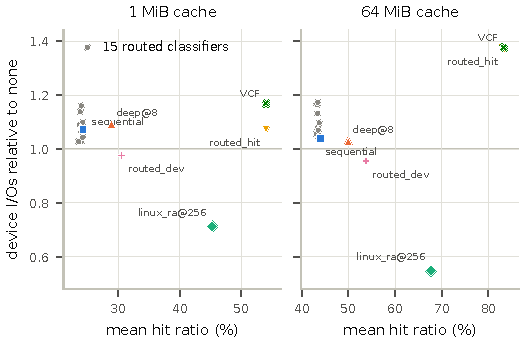
\includegraphics[width=\columnwidth]{figures/f9_action_space}
\caption{The action-space ceiling (simulated, C3 slice 2, \clfRouterTraces{}
traces): mean hit ratio against device I/Os relative to \texttt{none}. The
\clfRouterClassifiers{} routed classifiers sit with \texttt{sequential};
depth, window growth and the hindsight routers move away from it. VCF is the
validation-chosen fixed action.}
\label{fig:f9}
\end{figure}

\textbf{Routing real traces} (Fig.~\ref{fig:f9},
Table~\ref{tab:t11_classifier_router}). By the claim rule,
\decClfClaimBeatsReadAheadOneMiBVerdict{} at either capacity: all
\decTallyClfOneOneMiB{} show no difference detected against
\texttt{sequential} at 1\,MiB and all are worse at 64\,MiB (the best, an MLP,
by \decClfOneMlpSixtyFourMiBPairedCI). Against the shipped GNB, only the random
forest is better at 1\,MiB (\decClfTwoRfOneMiBPairedCI{} paired,
\decClfTwoRfOneMiBClusterCI{} cluster), and \decTallyClfTwoSixtyFourMiBBetter{}
of \decTallyClfTwoSixtyFourMiB{} alternatives are at 64\,MiB. Every routed
classifier increases device I/Os (\clfRouterIORatioMinOneMiB--\clfRouterIORatioMaxOneMiB{}
of \texttt{none}'s at 1\,MiB), while \texttt{linux\_ra@256} adds
\decClfOneLinuxRaAtTwoHundredFiftySixOneMiBPaired{} over \texttt{sequential}
with \clfRouterIORatioLinuxRaAtTwoHundredFiftySixOneMiB{} of the I/Os. The
classifiers agree with GNB on only \clfRouterAgreementMin--\clfRouterAgreementMax{}
of windows, yet the hit ratio barely moves: the class decides little when
every class prefetches two blocks at most.

\textbf{Depth as an action.} The hindsight router picks the next window's
action among \texttt{none}, \texttt{sequential}, \texttt{deep@8},
\texttt{deep@32} and \texttt{deep@256}. Its label is the action that did best
on that window in its own fixed replay, a trajectory approximation in the
spirit of hindsight-labelled caching~\cite{jain2016hawkeye} and open to the
distribution shift of imitation learning~\cite{ross2011reduction}. We selected
among \hsrCvFamilies{} families by corpus-grouped cross-validation on the
first slice and scored the second (Table~\ref{tab:t12_hindsight}). Against the
per-trace validation-chosen fixed action (VCF), the router shows
\decHsrHOneHitRatioRoutedHitVsVcfHitOneMiBVerdict{} at 1\,MiB
(\decHsrHOneHitRatioRoutedHitVsVcfHitOneMiBPairedCI) and is
\decHsrHOneHitRatioRoutedHitVsVcfHitSixtyFourMiBVerdict, by a negligible
\decHsrHOneHitRatioRoutedHitVsVcfHitSixtyFourMiBPaired, at 64\,MiB, where it
sends \hsrDeepShareRoutedHitSixtyFourMiB{} of windows to \texttt{deep@256}, the
VCF action. Its gains over \texttt{sequential}
(\decHsrHTwoHitRatioRoutedHitVsSequentialOneMiBPaired{} at 1\,MiB) and
\texttt{linux\_ra@256} are depth's, at \hsrMovedRatioRoutedHitOneMiB{} the
blocks moved by \texttt{none}. A device-objective router
\decHsrDDeviceIosRoutedDevVsNoneOneMiBVerdict{}
(\decHsrDDeviceIosRoutedDevVsNoneOneMiBPaired{} of \texttt{none}'s), but
\texttt{linux\_ra@256} needs only \hsrIORatioLinuxRaAtTwoHundredFiftySixOneMiB.
GNB had the lowest cross-validation score in \hsrCvGnbLowest{} of
\hsrCvCells{} cells, yet the best family does not beat VCF; nor is the
trajectory oracle a true ceiling, since it beats VCF at 1\,MiB only.

\textbf{Web rankers} (Table~\ref{tab:t13_web_rankers}). On the same candidates
and features, tuned boosting, forests, extra trees and an MLP rank better than
the shipped logistic ranker (MLP: \decWrkKOneMlpMrrAtEightCI{} in MRR@8). By the
primary rule, \decWrkRuleTwoCapEightVerdict{} at both capacities, the one
learned predictor here that does: the validation-selected MLP raises $U(c)$ per
view at $c$ = \webHeadlineCost{} by \decWrkSOneMlpUtilityPerViewCapEightCI{} at
capacity 8 and \decWrkSOneMlpUtilityPerViewCapThirtyTwoCI{} at 32, though its
hit ratio at capacity 8 is lower (\decWrkSOneMlpHitRatioCapEightCI). No family
beats transition top-1 at depth 1, and all stay far below online counts (MLP:
\decWrkKFiveMlpHitRatioCapEightCI): a better ranker does not close the
freshness gap.
